\chapter{Survey Modelling}

Space missions are very expensive to design, build, launch and operate. Therefore, it is important that all properties and behaviors of such a mission are well known in advance. Then, an accurate assessment can be made of the merits of the mission and what results are to be expected. In addition, it allows for selecting the design which will produce the best results. In order to study these properties and determine the optimum, computer simulations are an excellent tool. They allow for cheaply and rapidly testing out a lot of possible mission parameters, and recording the relevant data for easy analysis. \\

\begin{figure}[htbp]
 \centering
 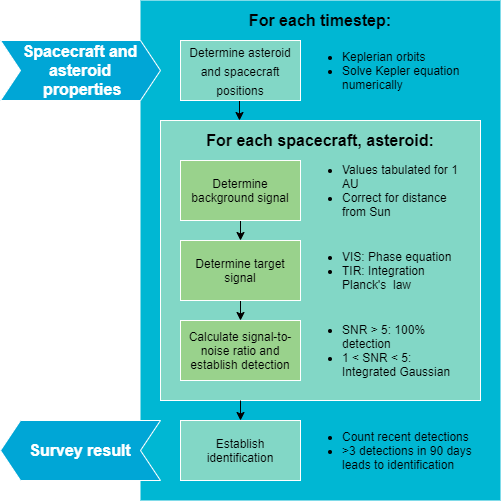
\includegraphics[width=0.7\textwidth]{img/simulation_overview.png}
 \caption{Overview of the simulation architecture and main loops.}
 \label{fig:simulation_overview}
\end{figure}

Currently, no model is publicly available for modelling multi-spacecraft surveys. Therefore, a simulation will be developed. During and after development, the model is also extensively verified and validated. The process for this is described in REF??. Other research (e.g. \cite{Flyeye}, \cite{2017NEOSDT}) has demonstrated the potential for explicitly modelling out the entire survey as it would be conducted by the actual system. This consists of first generating a representative population of asteroids (described in \autoref{sec:modelling_population}), then, at each timestep, calculating the background and target signal (\autoref{sec:modelling_background} and \autoref{sec:modelling_target}, respectively). Knowing these signals, the signal-to-noise ratios can then be determined after estimation of some of the detector properties (\autoref{sec:modelling_hardware_SNR}). The frequency and location of the observations is determined by the search strategy, and resulting cadence (detailed in \autoref{sec:modelling_cadence}) and lastly through repeat observations, it can be determined whether the system is capable of identifying a target (\autoref{sec:modelling_identification}).\\


The architecture of the simulation is shown in \autoref{fig:simulation_overview}. On the top left, the main input parameters to the model are displayed. These are primarily the spacecraft and asteroid properties. Both of these consist of a full set of Keplerian orbital elements per spacecraft or asteroid. The asteroid properties furthermore include the albedo, size, and absolute magnitude of each asteroid; the spacecraft properties include which type of payload the spacecraft is carrying. \\

The simulation consists of a nested loop. Firstly, at the start of each timestep (the time between the timesteps is determined by the survey cadence), the positions of all asteroids and spacecraft are determined by propagation of their orbital elements. Then, in the inside loop, each spacecraft is checked against each asteroid to see if it can detect said asteroid. This is done through calculation of the signal-to-noise ratio (SNR). Lastly, as it is known which asteroids got succesfully detected by which spacecraft, it can be determined if asteroids have been identified. Then, at the end of the simulation, the result is a list of the asteroid population in addition to whether they have been detected, and if so, when. Of course, this data can be further processed.

\section{Population of Asteroids}
\label{sec:modelling_population}
The first component of the simulation is the asteroid population model. This population was already briefly described in \autoref{sec:introduction_NEA}. In this section, more details on the generation of the population and the process of determining the positions of the NEA's, are given. As already mentioned in \autoref{sec:introduction_NEA}, the most comprehensive debiased population model is the one by \cite{PopulationGranvik}. This population model was generated by propagating an intiial population of NEA's based on several known interactions (e.g. gravitational interaction with the planets), and then comparing the resulting population to the results of the NEOWISE mission. Essentially, the problem then reduces to the question: ``What initial population would result in the results that are observed in the NEOWISE mission?''. Then, the initial population model can be fitted to the results of the NEOWISE mission, and an accurate population model is obtained. \\

Of course, this results in a full population of NEA's; whereas a population of \textit{unidentified} NEA's is required for this work. Therefore, a correction to the population was made based on the work of \cite{PopulationHarris}. To do this, the population as given by \cite{PopulationGranvik} was separated, based on absolute magnitude, into bins of width 0.5. Then, it was assumed that the detection of NEAs is roughly uniform over the orbital parameters. The completeness statistics of \cite{PopulationHarris} can then be used to discard a part of the population as \textit{identified}. For example, given 10000 asteroids in the bin width XXYYZZ, where 70\% is considered identified at this time, 7000 asteroids are selected at random and discarded. Of course, the assumption of uniformity in the detection of NEA's is false: highly eccentric NEA's, NEA's that are very dark, or NEA's with a high semi-major axis are more likely to be undetected. However, no data is available on this matter, and therefore no better alternative was deemed to be available. As all simulations will be affected equally, the error is judged to be sufficiently small for practical purposes.

\section{Background Signal}
\label{sec:modelling_background}

\section{Target Signal}
\label{sec:modelling_target}

\section{Hardware Properties and Signal-to-Noise Ratio}
\label{sec:modelling_hardware_SNR}

\section{Search Strategy and Cadence}
\label{sec:modelling_cadence}

\section{Detection and Identification}
\label{sec:modelling_identification}
